\section{Project Management}
Due to this project being spread over almost an entire year, a certain amount of management needs to be maintained in order to ensure that work does not fall behind.

\subsection{Gannt Chart}
One method used in this project to keep track of things is a Gannt Chart.
This is a way of showing what work should be being done when, and allowing thinkgs over running to be easily noticed.

\begin{figure}[h]
	\centering
	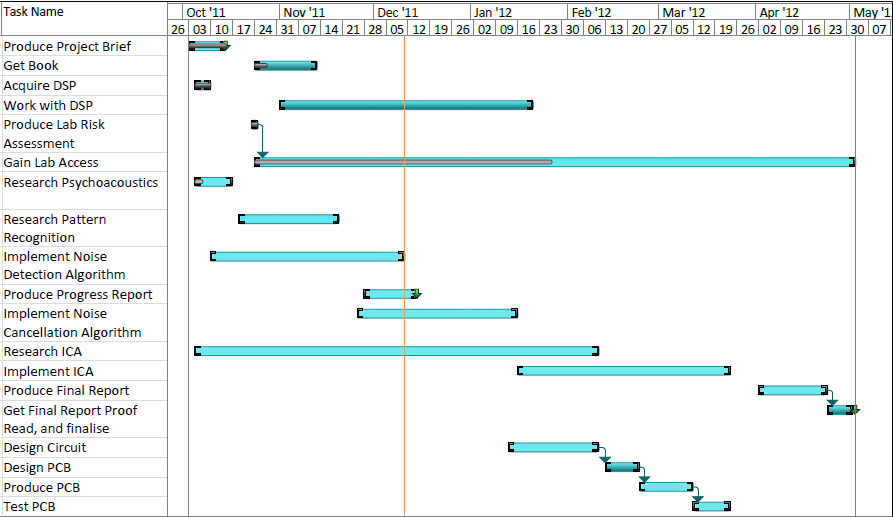
\includegraphics[width=\textwidth]{./img/ganntori.png}
	\caption{The Gannt chart for this project as originally produced}
	\label{fig:gannt}
\end{figure}

This Gannt chart changes regularly as time gets reallocated and tasks get completed ahead or behind schedule.
The current up to date version of this chart can be seen in figure~\ref{fig:newgannt}

\begin{figure}[H]
	\centering
	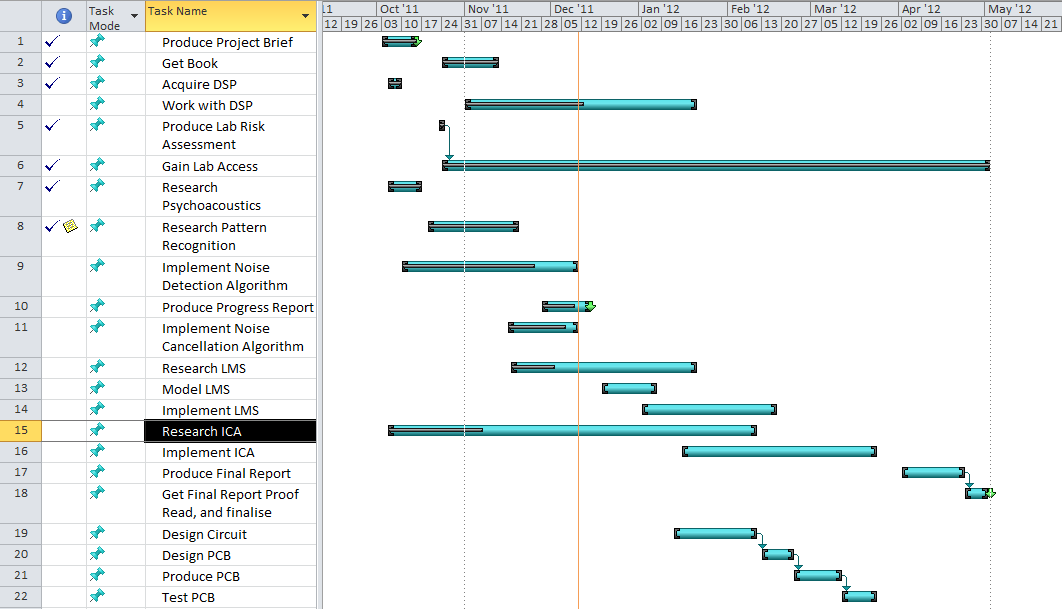
\includegraphics[width=\textwidth]{./img/ganntnew.png}
	\caption{The up to date Gannt chart for this project}
	\label{fig:newgannt}
\end{figure}

A few differences can be seen between these.
The majority of the differences are tasks that have been achieved, however the most significant difference is the introduction of the sections on LMS which will be discussed in section~\ref{sec:LMS}.

\subsection{Weekly Tracker}
While Gannt Charts clearly show what should be being done when, I felt it would help me more to have a shorter term list of things that needed doing, and a way of measuring how well on track I was at the time. As such I created the 'Weekly Tracker'.
The weekly tracker was a sheet containing a list of tasks to work on during the coming week, including a review date on which I would look back and see how well I'd kept up. Each tracking sheet also included a weekly score.

Each task has a task name, also it had space for notes at the beginning and end of the week. Along with this, each task has a rank from 0 to 10 for minimum acceptable completion. This is essentially the minimum percentage of the task that I need to have completed by the end of the week to remain on track. Using a rank below 10 here allows for tasks to cross multiple weeks, with increasing the required rank as progressing through the project.
There is also a rank for task completion. This rank is out of the entire task, not just the amount required for the week allowing me to note if I had progressed beyond where expected for that week. In the event that I progressed beyond the scope required by the overall task, I would be able to rank this as '+'.
At the end of the week, after completing the ranks for task completion, I could then sum up the differences between required and completed ranks to give me a score for the week.
A negative score would denote that I am behind schedule, a positive score denotes that I'm ahead of schedule, and a score of 0 would indicate that I'm spot on schedule.

\subsection{Milestones}
In order to determine the state of the system a collection of milestones has been set.
At each one the system would be able to demonstrate a level of functionality.
This would allow any major progress in the system would be noted and, in the event of something preventing the project being completed, these milestones would allow the progress of the system to still be observed.
Each of these milestones has a list of requirements required to be met before they can be classed as achieved.
These milestones are shown in table~\ref{tab:milestones}, however the requirements to meet the milestone are not shown.
These milestones do not have to be met in the order stated, and some of them will be worked on in parallel, though in most cases the milestones build on the previous ones.

\begin{table}[H]
	\centering
	\begin{tabular}[c]{| c | l | c |}
		\hline
		No.	& Milestone		& Achieved? \\
		\hline
		1	& Record/replay audio	& X \\
		2	& Cancellation algorithm & X \\
		3	& Cancellation on DSP	& X \\
		4	& Create PCB		& \\
		5	& LMS algorithm		& \\
		6	& LMS on DSP		& \\
		7	& Add ICA		& \\
		\hline
	\end{tabular}
	\caption{The milestones set for the project}
	\label{tab:milestones}
\end{table}
